%===================================== CHAP 6 =================================

\chapter{Results}
\section{BFS search}
BFS search without any pruning and search depth of 3 were unable to finish due to memory constraints and taking too long. Search with a depth of 2 may finish, depending on on the connectedness of the nodes discovered, and the amount of root nodes found in the search.

\subsection{Time}
When running the query, two sets are displayed, one with mostly random input data, and one with more closely selected data.

Because most of the randomly selected places had few possible root nodes, the table contains only the manually selected.

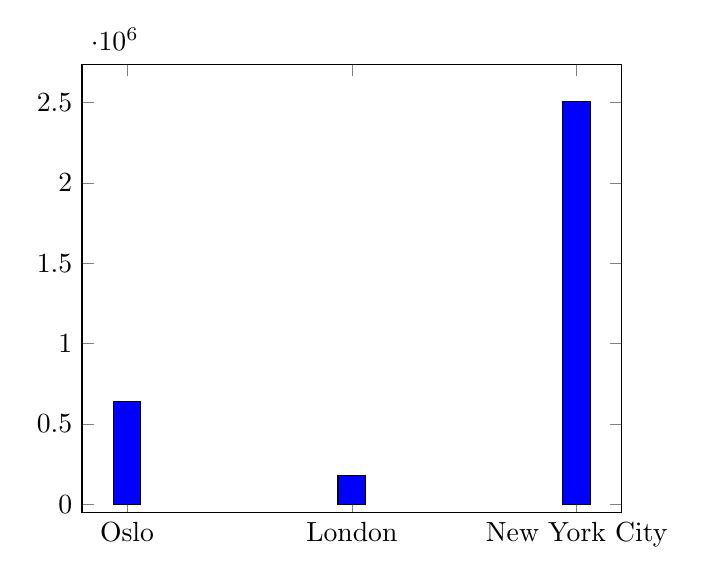
\begin{tikzpicture}
    \begin{axis}[
        symbolic x coords={Oslo, London, New York City},
        xtick=data
      ]
        \addplot[ybar,fill=blue] coordinates {
            (Oslo,   640106)
            (London,   181004)
            (New York City,   2507057)
        };
    \end{axis}
\end{tikzpicture}

\subsection{Accuracy}

\clearpage